% tikzpic.teP
\documentclass[crop,tikz]{standalone}% 'crop' is the default for v1.0, before it was 'preview'


%Packages
\usepackage{xcolor}
\usepackage{bm}
\usepackage{amsmath}

%tikz libraries}}
\usetikzlibrary{arrows.meta}
\usetikzlibrary{shapes.geometric}
% \tikzset{custom={latex[length=2in,width=2mm]}}

%Colors
\definecolor{susceptible}{RGB}{141,160,203}
\definecolor{recovery}{RGB}{102,194,165}
\definecolor{infection}{RGB}{252,141,98}
\definecolor{intervention}{RGB}{50, 102, 86}
\definecolor{nothing}{RGB}{225,225,225}

% Formatting macros:
\tikzstyle{node}=[circle, draw]
\tikzstyle{edge}=[diamond, draw]

\tikzstyle{intervention}=[fill = intervention]
\tikzstyle{contact}=[fill = infection]
\tikzstyle{recovery}=[fill = recovery]
\tikzstyle{custom}=[-{Latex[scale=1,length=1.5mm,width=1.5mm]},color=black!40!white]

\begin{document}


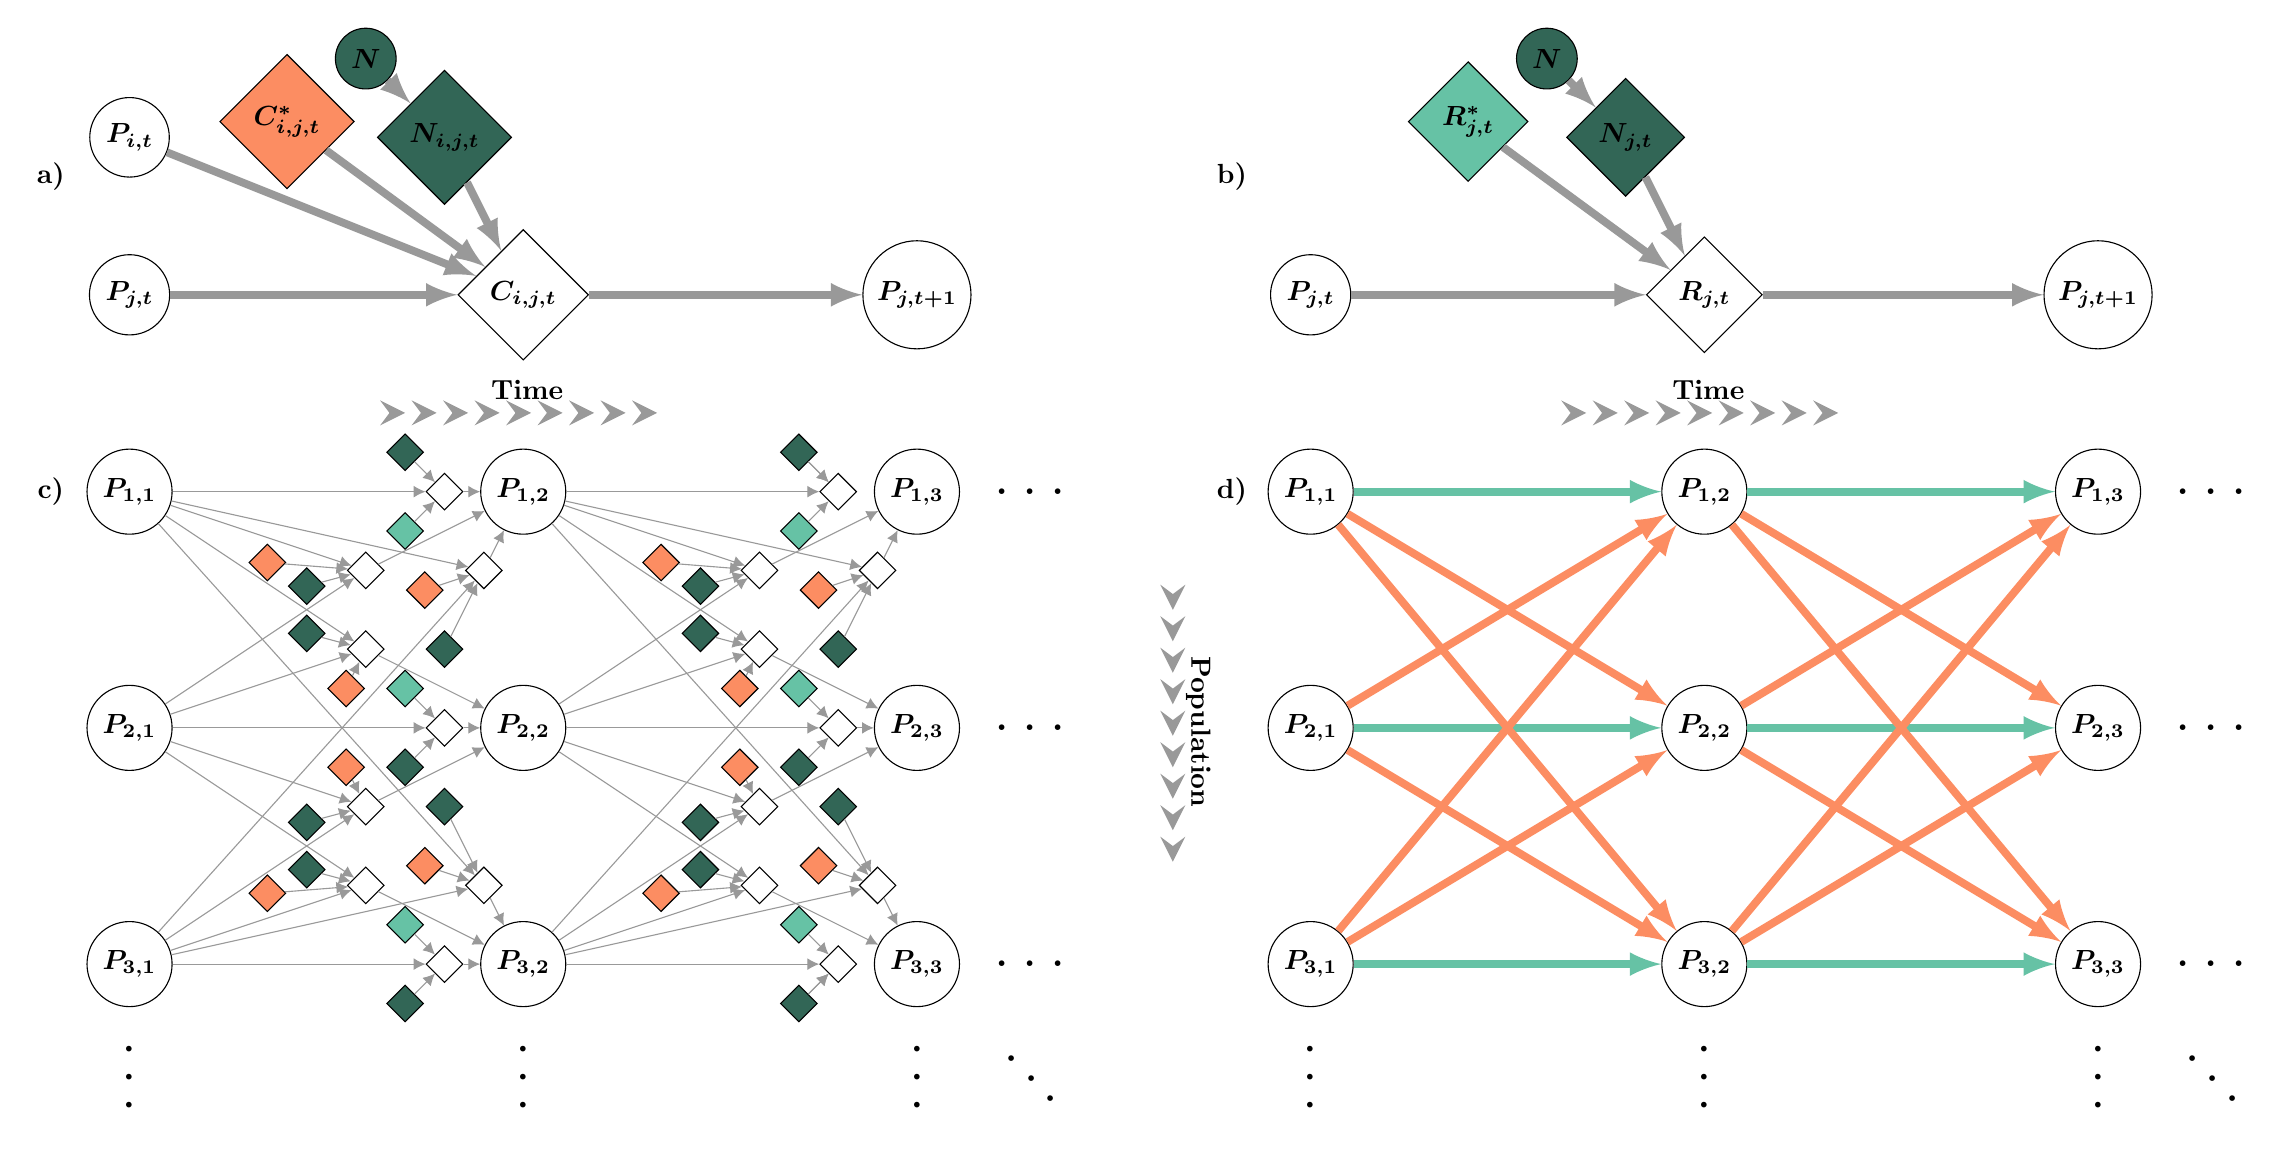
\begin{tikzpicture}
  %% Infectious Contacts
  \draw (-15,2.5) node[node] (P11) {$\bm{\bm{P_{i,t}}}$};
  \draw (-15,0.5) node[node] (P21) {$\bm{\bm{P_{j,t}}}$};
  \draw (-13,2.7) node[edge, contact] (E121) {$\bm{C^*_{i,j,t}}$};
  \draw (-12,3.5) node[node,intervention] (I) {$\bm{N}$};
  \draw (-11,2.5) node[edge, intervention] (I121) {$\bm{N_{i,j,t}}$};
  \draw (-5,0.5) node[node] (P22) {$\bm{P_{j,t+1}}$};
  \draw (-10,0.5) node[edge] (C121) {$\bm{C_{i,j,t}}$};
  
  \draw[-latex,color=black!40!white,line width=1mm] (P11) -- (C121);
  \draw[-latex,color=black!40!white,line width=1mm] (P21) -- (C121);
  \draw[-latex,color=black!40!white,line width=1mm] (C121) -- (P22);
  \draw[-latex,color=black!40!white,line width=1mm] (E121) -- (C121);
  \draw[-latex,color=black!40!white,line width=1mm] (I121) -- (C121);
  \draw[-latex,color=black!40!white,line width=1mm] (I) -- (I121);
  
  
  %% Recovery
  \draw (0,0.5) node[node] (P21) {$\bm{P_{j,t}}$};
  \draw (2,2.7) node[edge, recovery] (E121) {$\bm{R^*_{j,t}}$};
  \draw (3,3.5) node[node, intervention] (I) {$\bm{N}$};
  \draw (4,2.5) node[edge, intervention] (I11) {$\bm{N_{j,t}}$};
  \draw (10,0.5) node[node] (P22) {$\bm{P_{j,t+1}}$};
  \draw (5,0.5) node[ edge] (R121) {$\bm{R_{j,t}}$};
  
  \draw[-latex,color=black!40!white,line width=1mm] (P21) -- (R121);
  \draw[-latex,color=black!40!white,line width=1mm] (R121) -- (P22);
  \draw[-latex,color=black!40!white,line width=1mm] (E121) -- (R121);
  \draw[-latex,color=black!40!white,line width=1mm] (I11) -- (R121);
  \draw[-latex,color=black!40!white,line width=1mm] (I) -- (I11);
  
  
  %% Full
  \draw (-15,-5) node[node] (P11) {$\bm{P_{2,1}}$};
  \draw (-15,-8) node[node] (P21) {$\bm{P_{3,1}}$};
  \draw (-15,-2) node[node] (P31) {$\bm{P_{1,1}}$};

  \draw (-10,-5) node[node] (P12) {$\bm{P_{2,2}}$};
  \draw (-10,-8) node[node] (P22) {$\bm{P_{3,2}}$};
  \draw (-10,-2) node[node] (P32) {$\bm{P_{1,2}}$};

  \draw (-5,-5) node[node] (P13) {$\bm{P_{2,3}}$};
  \draw (-5,-8) node[node] (P23) {$\bm{P_{3,3}}$};
  \draw (-5,-2) node[node] (P33) {$\bm{P_{1,3}}$};

  %%% Contact edges
  \draw (-11.25,-6.75) node[edge,contact] (E321) {};
  \draw (-11.25,-3.25) node[edge,contact] (E231) {};
  \draw (-10.5,-7) node[edge] (C321) {};
  \draw (-10.5,-3) node[ edge] (C231) {};
  \draw (-11,-6) node[edge,intervention] (I321) {};
  \draw (-11,-4) node[edge,intervention] (I231) {};

  \draw (-12.25,-4.5) node[edge,contact] (E311) {};
  \draw (-13.25,-2.9) node[edge,contact] (E131) {};
  \draw (-12,-4) node[edge] (C311) {};
  \draw (-12,-3) node[ edge] (C131) {};
  \draw (-12.75,-3.8) node[edge,intervention] (I311) {};
  \draw (-12.75,-3.2) node[edge,intervention] (I131) {};

  \draw (-13.25,-7.1) node[edge,contact] (E121) {};
  \draw (-12.25,-5.5) node[edge,contact] (E211) {};
  \draw (-12,-7) node[edge] (C121) {};
  \draw (-12,-6) node[ edge] (C211) {};
  \draw (-12.75,-6.8) node[edge,intervention] (I121) {};
  \draw (-12.75,-6.2) node[edge,intervention] (I211) {};
  
  \draw (-11.5,-2.5) node[edge,recovery] (E31) {};
  \draw (-11.5,-1.5) node[edge,intervention] (I31) {};
  \draw (-11,-2) node[edge] (R31) {};
  \draw (-11.5,-7.5) node[edge,recovery] (E21) {};
  \draw (-11.5,-8.5) node[edge,intervention] (I21) {};
  \draw (-11,-8) node[edge] (R21) {};
  \draw (-11.5,-4.5) node[edge,recovery] (E11) {};
  \draw (-11.5,-5.5) node[edge,intervention] (I11) {};
  \draw (-11,-5) node[edge] (R11) {};

  \draw (-6.25,-6.75) node[edge,contact] (E322) {};
  \draw (-6.25,-3.25) node[edge,contact] (E232) {};
  \draw (-5.5,-7) node[edge] (C322) {};
  \draw (-5.5,-3) node[ edge] (C232) {};
  \draw (-6,-6) node[edge,intervention] (I322) {};
  \draw (-6,-4) node[edge,intervention] (I232) {};

  \draw (-7.25,-4.5) node[edge,contact] (E312) {};
  \draw (-8.25,-2.9) node[edge,contact] (E132) {};
  \draw (-7,-4) node[edge] (C312) {};
  \draw (-7,-3) node[ edge] (C132) {};
  \draw (-7.75,-3.8) node[edge,intervention] (I312) {};
  \draw (-7.75,-3.2) node[edge,intervention] (I132) {};

  \draw (-8.25,-7.1) node[edge,contact] (E122) {};
  \draw (-7.25,-5.5) node[edge,contact] (E212) {};
  \draw (-7,-7) node[edge] (C122) {};
  \draw (-7,-6) node[ edge] (C212) {};
  \draw (-7.75,-6.8) node[edge,intervention] (I122) {};
  \draw (-7.75,-6.2) node[edge,intervention] (I212) {};
  
  \draw (-6.5,-2.5) node[edge,recovery] (E32) {};
  \draw (-6.5,-1.5) node[edge,intervention] (I32) {};
  \draw (-6,-2) node[edge] (R32) {};
  \draw (-6.5,-7.5) node[edge,recovery] (E22) {};
  \draw (-6.5,-8.5) node[edge,intervention] (I22) {};
  \draw (-6,-8) node[edge] (R22) {};
  \draw (-6.5,-4.5) node[edge,recovery] (E12) {};
  \draw (-6.5,-5.5) node[edge,intervention] (I12) {};
  \draw (-6,-5) node[edge] (R12) {};


  \draw (-3.5,-2) node{\Huge \dots};
  \draw (-3.5,-5) node{\Huge \dots};
  \draw (-3.5,-8) node{\Huge \dots};

  \draw (-15,-9.5) node[rotate=-90]{\Huge \dots};
  \draw (-10,-9.5) node[rotate=-90]{\Huge \dots};
  \draw (-5,-9.5) node[rotate=-90]{\Huge \dots};
  \draw (-3.5,-9.5) node[rotate=-45]{\Huge \dots};

  % \draw (-8.5,-5) node[edge,contact] (E132) {};
  % \draw (-8.5,-4) node[edge,contact] (E312) {};
  % \draw (-7,-5) node[ edge] (C132) {};
  % \draw (-7,-4) node[ edge] (C312) {};
  % \draw (-8,-4.75) node[edge,intervention] (I132) {};
  % \draw (-8,-4.25) node[edge,intervention] (I312) {};
  % 
  % \draw (-6.5,-8) node[edge,recovery] (E32) {};
  % \draw (-7,-7.75) node[edge,intervention] (I32) {};
  % \draw (-6,-7.5) node[edge] (R32) {};

  \draw[custom] (P31) -- (C311);
  \draw[custom] (P11) -- (C311);
  \draw[custom] (E311) -- (C311);
  \draw[custom] (I311) -- (C311);
  \draw[custom] (C311) -- (P12);

  \draw[custom] (P21) -- (C231);
  \draw[custom] (P31) -- (C231);
  \draw[custom] (E231) -- (C231);
  \draw[custom] (I231) -- (C231);
  \draw[custom] (C231) -- (P32);

  \draw[custom] (P31) -- (C321);
  \draw[custom] (P21) -- (C321);
  \draw[custom] (E321) -- (C321);
  \draw[custom] (I321) -- (C321);
  \draw[custom] (C321) -- (P22);

  \draw[custom] (P11) -- (C131);
  \draw[custom] (P31) -- (C131);
  \draw[custom] (E131) -- (C131);
  \draw[custom] (I131) -- (C131);
  \draw[custom] (C131) -- (P32);

  \draw[custom] (P11) -- (C121);
  \draw[custom] (P21) -- (C121);
  \draw[custom] (E121) -- (C121);
  \draw[custom] (I121) -- (C121);
  \draw[custom] (C121) -- (P22);

  \draw[custom] (P11) -- (C211);
  \draw[custom] (P21) -- (C211);
  \draw[custom] (E211) -- (C211);
  \draw[custom] (I211) -- (C211);
  \draw[custom] (C211) -- (P12);

  \draw[custom] (P11) -- (R11);
  \draw[custom] (P21) -- (R21);
  \draw[custom] (P31) -- (R31);
  \draw[custom] (E11) -- (R11);
  \draw[custom] (E21) -- (R21);
  \draw[custom] (E31) -- (R31);
  \draw[custom] (I11) -- (R11);
  \draw[custom] (I21) -- (R21);
  \draw[custom] (I31) -- (R31);
  \draw[custom] (R11) -- (P12);
  \draw[custom] (R21) -- (P22);
  \draw[custom] (R31) -- (P32);
  
  

  \draw[custom] (P22) -- (C232);
  \draw[custom] (P32) -- (C232);
  \draw[custom] (E232) -- (C232);
  \draw[custom] (I232) -- (C232);
  \draw[custom] (C232) -- (P33);

  \draw[custom] (P22) -- (C322);
  \draw[custom] (P32) -- (C322);
  \draw[custom] (E322) -- (C322);
  \draw[custom] (I322) -- (C322);
  \draw[custom] (C322) -- (P23);
  
  \draw[custom] (P12) -- (C132);
  \draw[custom] (P32) -- (C132);
  \draw[custom] (E132) -- (C132);
  \draw[custom] (I132) -- (C132);
  \draw[custom] (C132) -- (P33);

  \draw[custom] (P12) -- (C312);
  \draw[custom] (P32) -- (C312);
  \draw[custom] (E312) -- (C312);
  \draw[custom] (I312) -- (C312);
  \draw[custom] (C312) -- (P13);
  
  \draw[custom] (P12) -- (C122);
  \draw[custom] (P22) -- (C122);
  \draw[custom] (E122) -- (C122);
  \draw[custom] (I122) -- (C122);
  \draw[custom] (C122) -- (P23);

  \draw[custom] (P12) -- (C212);
  \draw[custom] (P22) -- (C212);
  \draw[custom] (E212) -- (C212);
  \draw[custom] (I212) -- (C212);
  \draw[custom] (C212) -- (P13);

  \draw[custom] (P12) -- (R12);
  \draw[custom] (P22) -- (R22);
  \draw[custom] (P32) -- (R32);
  \draw[custom] (E12) -- (R12);
  \draw[custom] (E22) -- (R22);
  \draw[custom] (E32) -- (R32);
  \draw[custom] (I12) -- (R12);
  \draw[custom] (I22) -- (R22);
  \draw[custom] (I32) -- (R32);
  \draw[custom] (R12) -- (P13);
  \draw[custom] (I22) -- (R22);
  \draw[custom] (I32) -- (R32);

  \draw (0,-2) node[node] (P11) {$\bm{P_{1,1}}$};
  \draw (0,-5) node[node] (P21) {$\bm{P_{2,1}}$};
  \draw (0,-8) node[node] (P31) {$\bm{P_{3,1}}$};

  \draw (5,-2) node[node] (P12) {$\bm{P_{1,2}}$};
  \draw (5,-5) node[node] (P22) {$\bm{P_{2,2}}$};
  \draw (5,-8) node[node] (P32) {$\bm{P_{3,2}}$};

  \draw (10,-2) node[node] (P13) {$\bm{P_{1,3}}$};
  \draw (10,-5) node[node] (P23) {$\bm{P_{2,3}}$};
  \draw (10,-8) node[node] (P33) {$\bm{P_{3,3}}$};

  \draw[-latex,line width=1mm, color=recovery] (P11) -- (P12);
  \draw[-latex,line width=1mm, color=recovery] (P21) -- (P22);
  \draw[-latex,line width=1mm, color=recovery] (P31) -- (P32);
  \draw[-latex,line width=1mm, color=infection] (P11) -- (P22);
  \draw[-latex,line width=1mm, color=infection] (P21) -- (P12);
  \draw[-latex,line width=1mm, color=infection] (P11) -- (P32);
  \draw[-latex,line width=1mm, color=infection] (P21) -- (P32);
  \draw[-latex,line width=1mm, color=infection] (P31) -- (P12);
  \draw[-latex,line width=1mm, color=infection] (P31) -- (P22);

  \draw[-latex,line width=1mm, color=recovery] (P12) -- (P13);
  \draw[-latex,line width=1mm, color=recovery] (P22) -- (P23);
  \draw[-latex,line width=1mm, color=recovery] (P32) -- (P33);
  \draw[-latex,line width=1mm, color=infection] (P12) -- (P23);
  \draw[-latex,line width=1mm, color=infection] (P22) -- (P13);
  \draw[-latex,line width=1mm, color=infection] (P12) -- (P33);
  \draw[-latex,line width=1mm, color=infection] (P22) -- (P33);
  \draw[-latex,line width=1mm, color=infection] (P32) -- (P13);
  \draw[-latex,line width=1mm, color=infection] (P32) -- (P23);

  \draw (11.5,-2) node{\Huge \dots};
  \draw (11.5,-5) node{\Huge \dots};
  \draw (11.5,-8) node{\Huge \dots};

  \draw (0,-9.5) node[rotate=-90]{\Huge \dots};
  \draw (5,-9.5) node[rotate=-90]{\Huge \dots};
  \draw (10,-9.5) node[rotate=-90]{\Huge \dots};
  \draw (11.5,-9.5) node[rotate=-45]{\Huge \dots};

  %% Legend thingies
  % \draw[-stealth,line width=1mm,white!60!black] (-12,-1) -- (-8,-1) node[midway, below,text=black] {\textbf{Time}};
  \draw[-stealth,line width=1mm,white!60!black] (-11.6,-1) -- (-11.5,-1) node[midway, above,text=black] {};
  \draw[-stealth,line width=1mm,white!60!black] (-11.2,-1) -- (-11.1,-1) node[midway, above,text=black] {};
  \draw[-stealth,line width=1mm,white!60!black] (-10.8,-1) -- (-10.7,-1) node[midway, above,text=black] {};
  \draw[-stealth,line width=1mm,white!60!black] (-10.4,-1) -- (-10.3,-1) node[midway, above,text=black] {};
  \draw[-stealth,line width=1mm,white!60!black] (-10.0,-1) -- (- 9.9,-1) node[midway, above,text=black] {\textbf{Time}};
  \draw[-stealth,line width=1mm,white!60!black] (- 9.6,-1) -- (- 9.5,-1) node[midway, above,text=black] {};
  \draw[-stealth,line width=1mm,white!60!black] (- 9.2,-1) -- (- 9.1,-1) node[midway, above,text=black] {};
  \draw[-stealth,line width=1mm,white!60!black] (- 8.8,-1) -- (- 8.7,-1) node[midway, above,text=black] {};
  \draw[-stealth,line width=1mm,white!60!black] (- 8.4,-1) -- (- 8.3,-1) node[midway, above,text=black] {};
  % \draw[-stealth,line width=1mm,white!60!black] (3,-1) -- (7,-1) node[midway, above,text=black] {\textbf{Time}};
  \draw[-stealth,line width=1mm,white!60!black] (3.4,-1) -- (3.5,-1) node[midway, above,text=black] {};
  \draw[-stealth,line width=1mm,white!60!black] (3.8,-1) -- (3.9,-1) node[midway, above,text=black] {};
  \draw[-stealth,line width=1mm,white!60!black] (4.2,-1) -- (4.3,-1) node[midway, above,text=black] {};
  \draw[-stealth,line width=1mm,white!60!black] (4.6,-1) -- (4.7,-1) node[midway, above,text=black] {};
  \draw[-stealth,line width=1mm,white!60!black] (5.0,-1) -- (5.1,-1) node[midway, above,text=black] {\textbf{Time}};
  \draw[-stealth,line width=1mm,white!60!black] (5.4,-1) -- (5.5,-1) node[midway, above,text=black] {};
  \draw[-stealth,line width=1mm,white!60!black] (5.8,-1) -- (5.9,-1) node[midway, above,text=black] {};
  \draw[-stealth,line width=1mm,white!60!black] (6.2,-1) -- (6.3,-1) node[midway, above,text=black] {};
  \draw[-stealth,line width=1mm,white!60!black] (6.6,-1) -- (6.7,-1) node[midway, above,text=black] {};
  % \draw[-latex,line width=1mm,white!60!black] (-1.75,-3) -- (-1.75,-7) node[midway, above,text=black,rotate=-90] {\textbf{Population}};
  \draw[-stealth,line width=1mm,white!60!black] (-1.75,-3.3) -- (-1.75,-3.5) node[midway, above,rotate=-90,text=black] {};
  \draw[-stealth,line width=1mm,white!60!black] (-1.75,-3.8) -- (-1.75,-3.9) node[midway, above,rotate=-90,text=black] {};
  \draw[-stealth,line width=1mm,white!60!black] (-1.75,-4.2) -- (-1.75,-4.3) node[midway, above,rotate=-90,text=black] {};
  \draw[-stealth,line width=1mm,white!60!black] (-1.75,-4.6) -- (-1.75,-4.7) node[midway, above,rotate=-90,text=black] {};
  \draw[-stealth,line width=1mm,white!60!black] (-1.75,-5.0) -- (-1.75,-5.1) node[midway, above,rotate=-90,text=black] {\textbf{Population}};
  \draw[-stealth,line width=1mm,white!60!black] (-1.75,-5.4) -- (-1.75,-5.5) node[midway, above,rotate=-90,text=black] {};
  \draw[-stealth,line width=1mm,white!60!black] (-1.75,-5.8) -- (-1.75,-5.9) node[midway, above,rotate=-90,text=black] {};
  \draw[-stealth,line width=1mm,white!60!black] (-1.75,-6.2) -- (-1.75,-6.3) node[midway, above,rotate=-90,text=black] {};
  \draw[-stealth,line width=1mm,white!60!black] (-1.75,-6.6) -- (-1.75,-6.7) node[midway, above,rotate=-90,text=black] {};
  %% Caption thingies
  \draw (-16,2) node{\textbf{a)}};
  \draw (-1,2) node{\textbf{b)}};
  \draw (-16,-2) node{\textbf{c)}};
  \draw (-1,-2) node{\textbf{d)}};
\end{tikzpicture}


\end{document}
